\chapter{Fondamenti teorici sugli impianti di automazione e robotica industriale}

\section{Contesto di Automazione industriale}
I sistemi autonomi in ambito industriale hanno trasformato e ridefinito il modo in cui le aziende gestiscono tutta la filiera dalla produzione al controllo dei processi. Grazie all'automazione è possibile eseguire operazioni altamente complesse in modo continuo, con alta precisione, affidabilità, e soprattutto riducendo al minimo l'intervento umano e il rischio di errore. Da qui nasce la possibilità di controllare impianti industriali di qualsiasi dimensione, oppure intere linee di produzione senza avere qualsiasi tipo di interruzione. Questo rappresenta un enorme vantaggio strategico per le aziende, perché permette di migliorare l'efficienza, la sicurezza e la qualità dei prodotti finiti. Tuttavia, automatizzare in modo corretto richiede un controllo in tempo reale e un sistema di monitoraggio che garantisca la consistenza dei parametri operativi, l'ottimizzazione delle risorse e soprattutto la possibilità di intervenire in modo immediato in caso di anomalie durante i processi.

In questo contesto nascono i sistemi SCADA (acronimo dall’inglese “Supervisory Control And Data Acquisition”, cioè “controllo di supervisione e acquisizione dati”), i quali hanno avuto un impatto determinante nella gestione e supervisione dei processi industriali. Ciò che li ha resi importanti è la loro capacità di raccogliere e analizzare dati in tempo reale, idealmente da un'ampia gamma di sensori e dispositivi presenti negli impianti. Questo permette di mantenere una visione d'insieme centralizzata delle operazioni, fondamentale per risolvere problematiche e ottimizzare i processi. Inoltre, l'esponenziale complessità delle operazioni industriali e soprattutto l'esigenza da parte dei clienti di massimizzare efficienza e sicurezza hanno reso i sistemi SCADA indispensabili: non solo permettono di monitorare e allo stesso tempo di controllare ogni singolo componente del sistema, ma supportano anche l'integrazione tra: impianti robotizzati, linee di produzione e altri sistemi autonomi, permettendo la creazione di un ecosistema interconnesso.\textsuperscript{\cite{sielcosistemi}} 

In breve, i sistemi SCADA sono diventati il cuore dell'automazione industriale moderna, garantendo gestione completa e affidabile delle operazioni, dall'acquisizione dei dati fino al controllo e intervento.

\section{Composizione di uno SCADA}
Un sistema SCADA è un sistema informatico distribuito (insieme di calcolatori interconnessi tra loro in un'architettura di tipo Client-Server, preposti a una o diverse funzionalità) che viene usato per il monitoraggio e la supervisione di sistemi fisici.

Un sistema SCADA di solito deve essere accompagnato da:
\begin{enumerate}
    \item Unità di acquisizione dati, dette anche: sensori ed attuatori che si occupano di misurare grandezze fisiche del sistema da controllare. Rappresentano il livello più basso della gerarchia SCADA.
    \item PLC (dall'inglese "Programmable Logic Controller"): è il componente più usato nelle reti industriali, si occupa di elaborare i dati provenienti dai sensori ed attuatori per poi eseguire il programma indicato, regolando le logiche di automazione dell'impianto. Comunica con tutto il sistema e monitora le grandezze interessate, mantenendo nei registri lo stato di tutte le variabili cui il sistema ha accesso.
    \item Sistema di telecomunicazione: è l'infrastruttura che consente di trasferire dati tra i vari dispositivi e il sistema centrale. È implementato attraverso protocolli di comunicazione come Modbus, Ethernet/IP e Profibus e si basa su reti cablate, wireless oppure satellitari, a seconda delle esigenze e della distanza dei dispositivi. Negli ultimi anni si predilige l'utilizzo di reti Ethernet e protocolli TCP/IP, poiché le grandi industrie necessitano di comunicare a grandi distanze.
    \item Un supervisore o HMI(dall'inglese "Human-Machine Interface"): un pannello o computer visibile agli operatori. Raccoglie dati dai microcontrollori tramite il sistema di telecomunicazione e li elabora, con l'obiettivo di fornire pieno controllo all'impianto (come ad esempio: far suonare allarmi se un insieme di parametri dovesse superare una valore limite). Attraverso l'HMI, l'operatore può monitorare, esaminare lo stato, analizzare gli storici ed interagire con il sistema in modo intuitivo.
\end{enumerate}
\begin{figure}
    \centering
    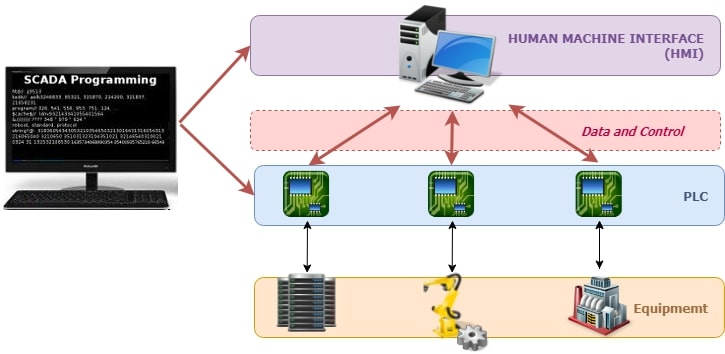
\includegraphics[width=0.7\linewidth]{Immagini/SCADA_system.jpg}
    \caption{Esempio sistema SCADA con componenti principali. Fonte: \cite{exonsys_scada}}
    \label{fig:SCADA_system.jpg}
\end{figure}

\section{Funzioni principali dello SCADA}
Un sistema SCADA svolge diverse funzioni chiave per assicurare una gestione efficace e sicura dei processi industriali, che differiscono da impianto ad impianto. Le fasi principali che generalmente uno SCADA dovrebbe fornire sono:
\begin{itemize}
    \item Acquisizione e raccolta dati: i sistemi SCADA acquisiscono dati dai dispositivi correlati di metadati e li trasferiscono al sistema centrale. Questo avviene in tempo reale per fornire continuamente consistenza sui vari parametri di processo.
    \item Visualizzazione e monitoraggio dei dati in tempo reale: i dati raccolti vengono rappresentati grazie all'HMI in formati intuitivi per favorire la lettura da parte degli operatori, attraverso grafici, tabelle interattive, led per allarmi e diagrammi di flusso.
    \item Archiviazione e storicizzazione del dato: vengono registrati i dati storici sia per analisi successive, sia per tenere traccia delle performance dell'impianto. Risultano essenziali per ottimizzare processi e per la manutenzione predittiva; inoltre i dati possono essere salvati su archivi locali o database relazionali, così da poter essere usufruibili sia tramite i formati sopra citati oppure esportati direttamente su sistemi esterni.
    \item Gestione eventi: un sistema SCADA genera allarmi e warning per segnalare criticità/anomalie nei parametri monitorati, sono una delle funzionalità cardine degli SCADA e richiedono sempre l'interazione con un operatore per evitare guasti o problemi di sicurezza. Inoltre tutti gli eventi vengono registrati e documentati per eventuali verifiche future.
    \item Controllo e manutenzione manuale: i sistemi SCADA oltre che a interfacciarsi con gli operatori, si interfacciano anche con l'impianto. Tale funzionalità è sempre più utilizzata e richiesta dai clienti per i sistemi SCADA, favorendo più flessibilità al sistema stesso, ma anche più complessità a livello progettuale.
\end{itemize}
\begin{figure}
    \centering
    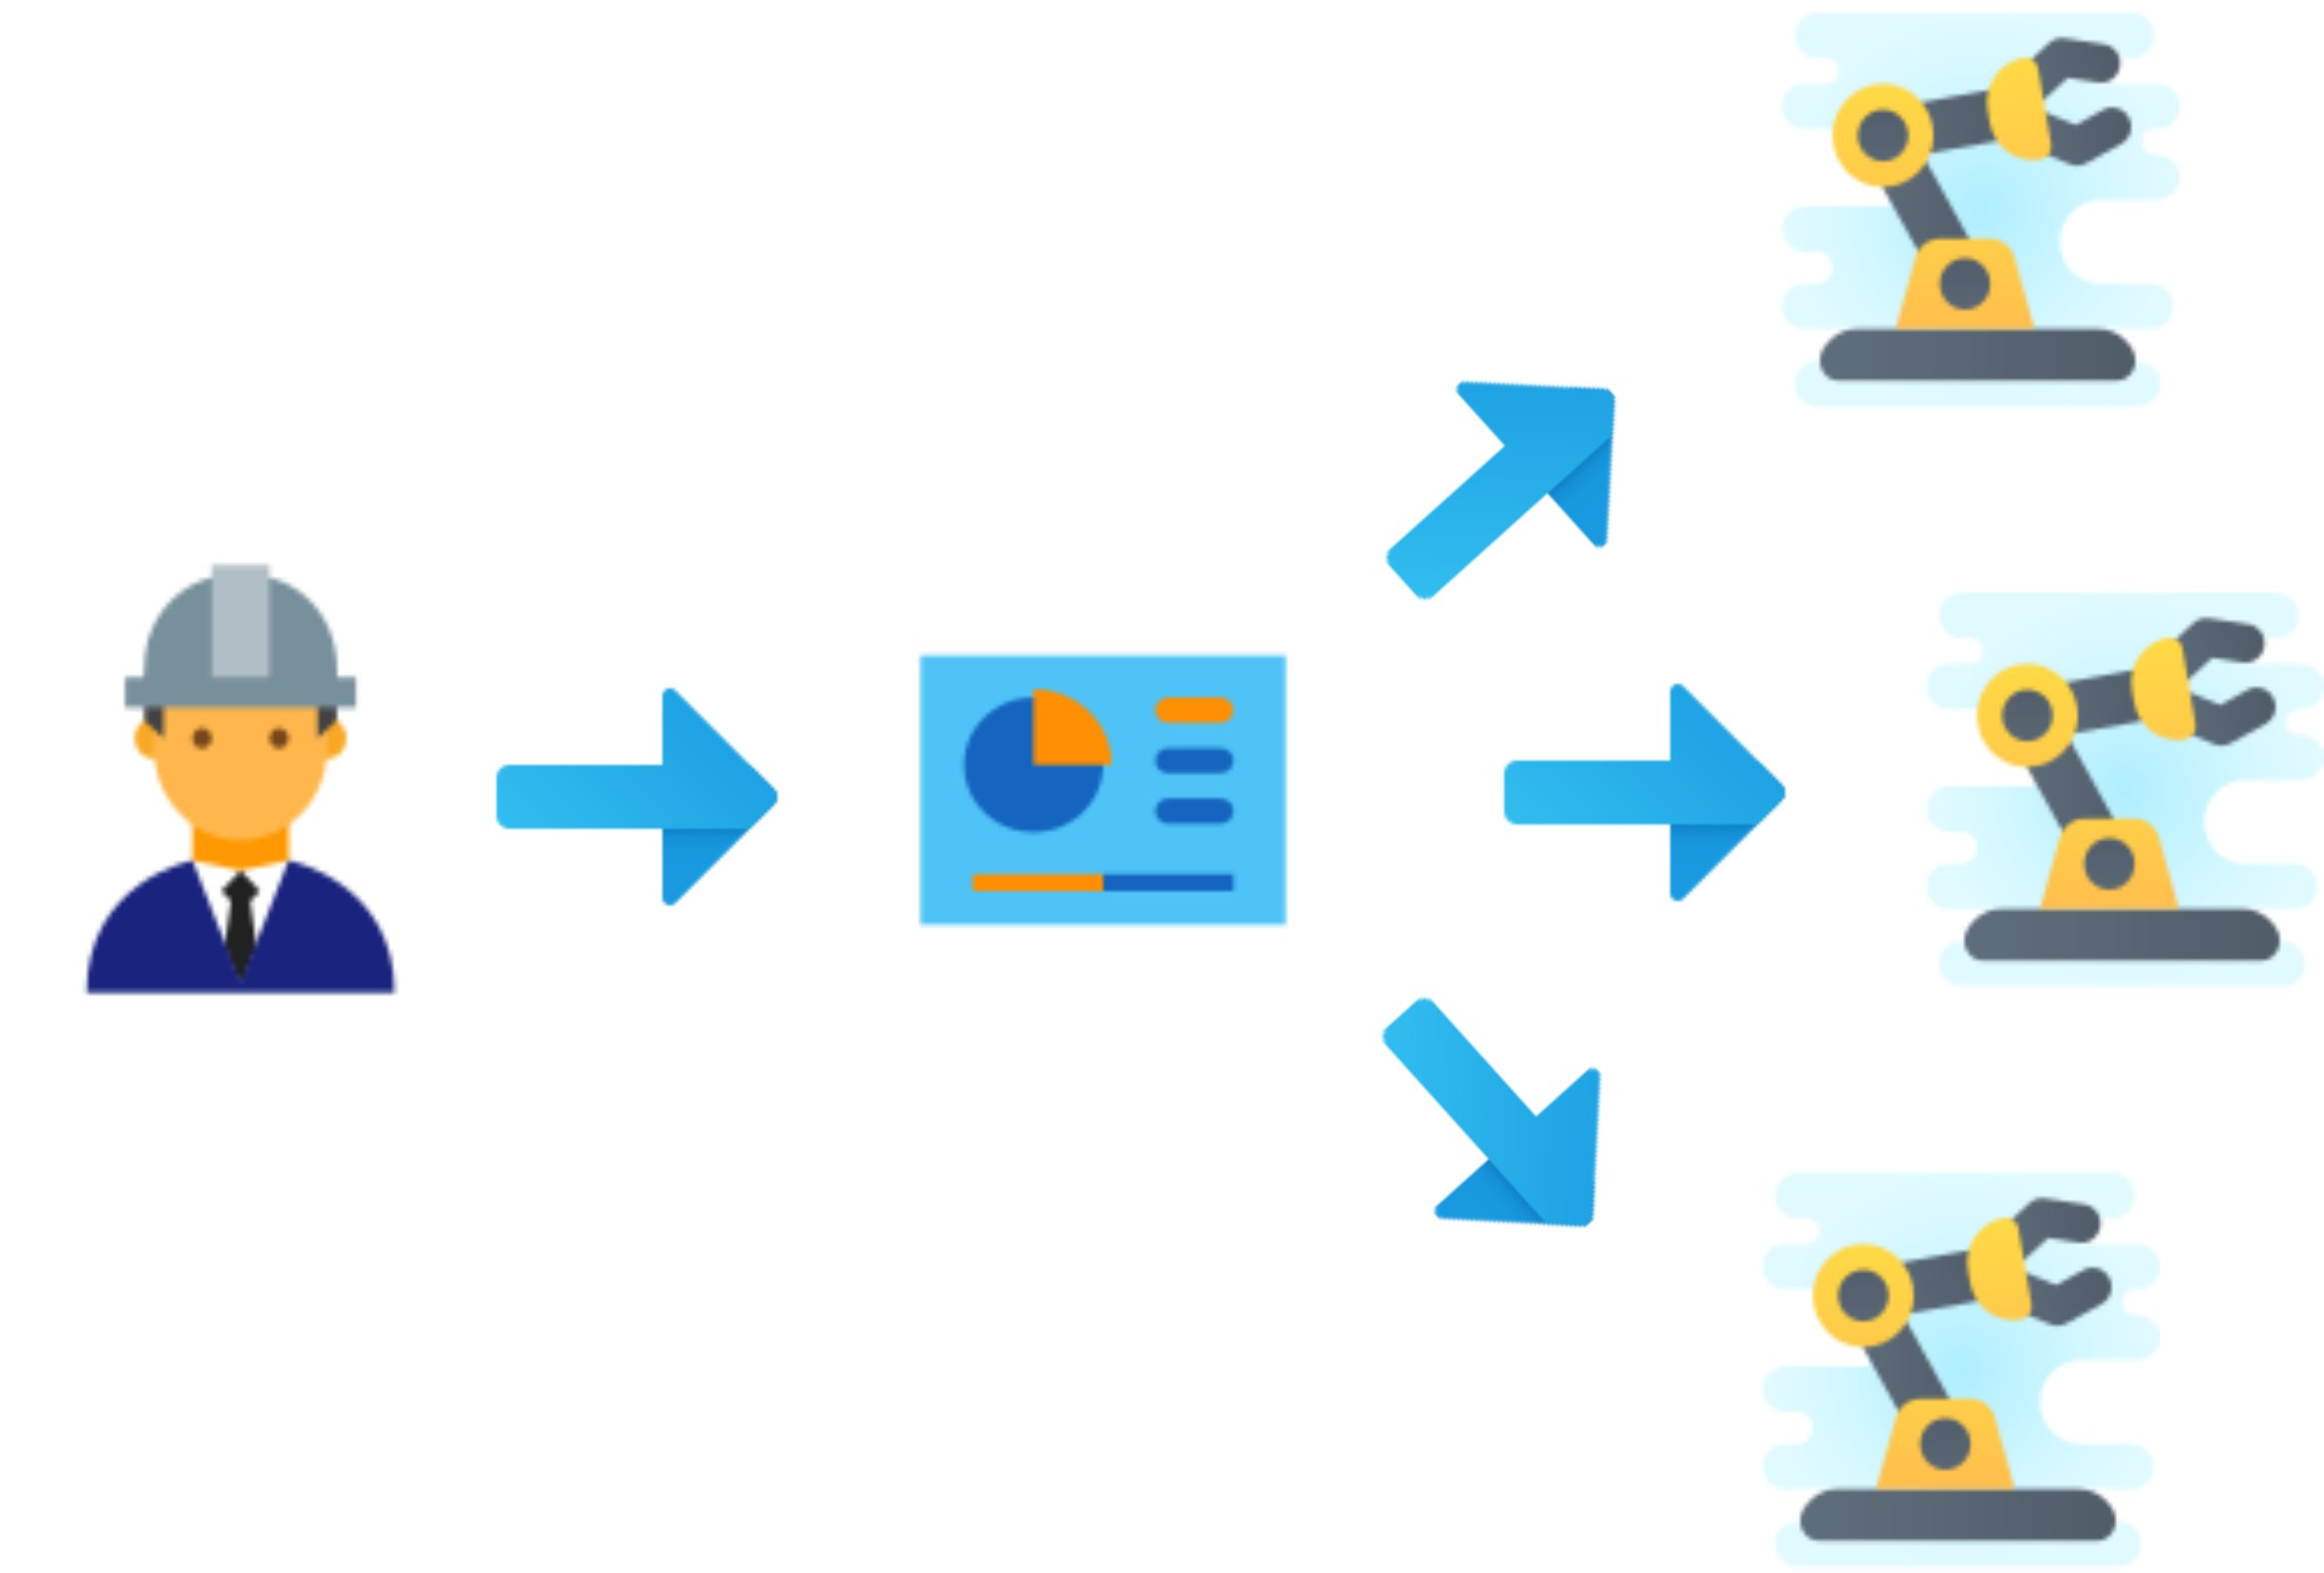
\includegraphics[width=0.5\linewidth]{Immagini/Operatore_SCADA.jpg}
    \caption{Gestione impianto tramite SCADA}
    \label{fig:Operatore_SCADA.jpg}
\end{figure}

\section{Piattaforma SCADA e Strumenti Software per la progettazione}
Con il termine piattaforma SCADA indichiamo solo lo strato software che svolge il lavoro definito in precedenza. Esistono diverse piattaforme che permettono di progettare un'interfaccia HMI per uno SCADA, e ognuna è affiancata dai propri linguaggi di programmazione proprietari, oppure i più famosi per poter progettare interfacce più avanzate (es: Jython, VBScript, C\#, ...)

\begin{figure} [ht]
    \centering
    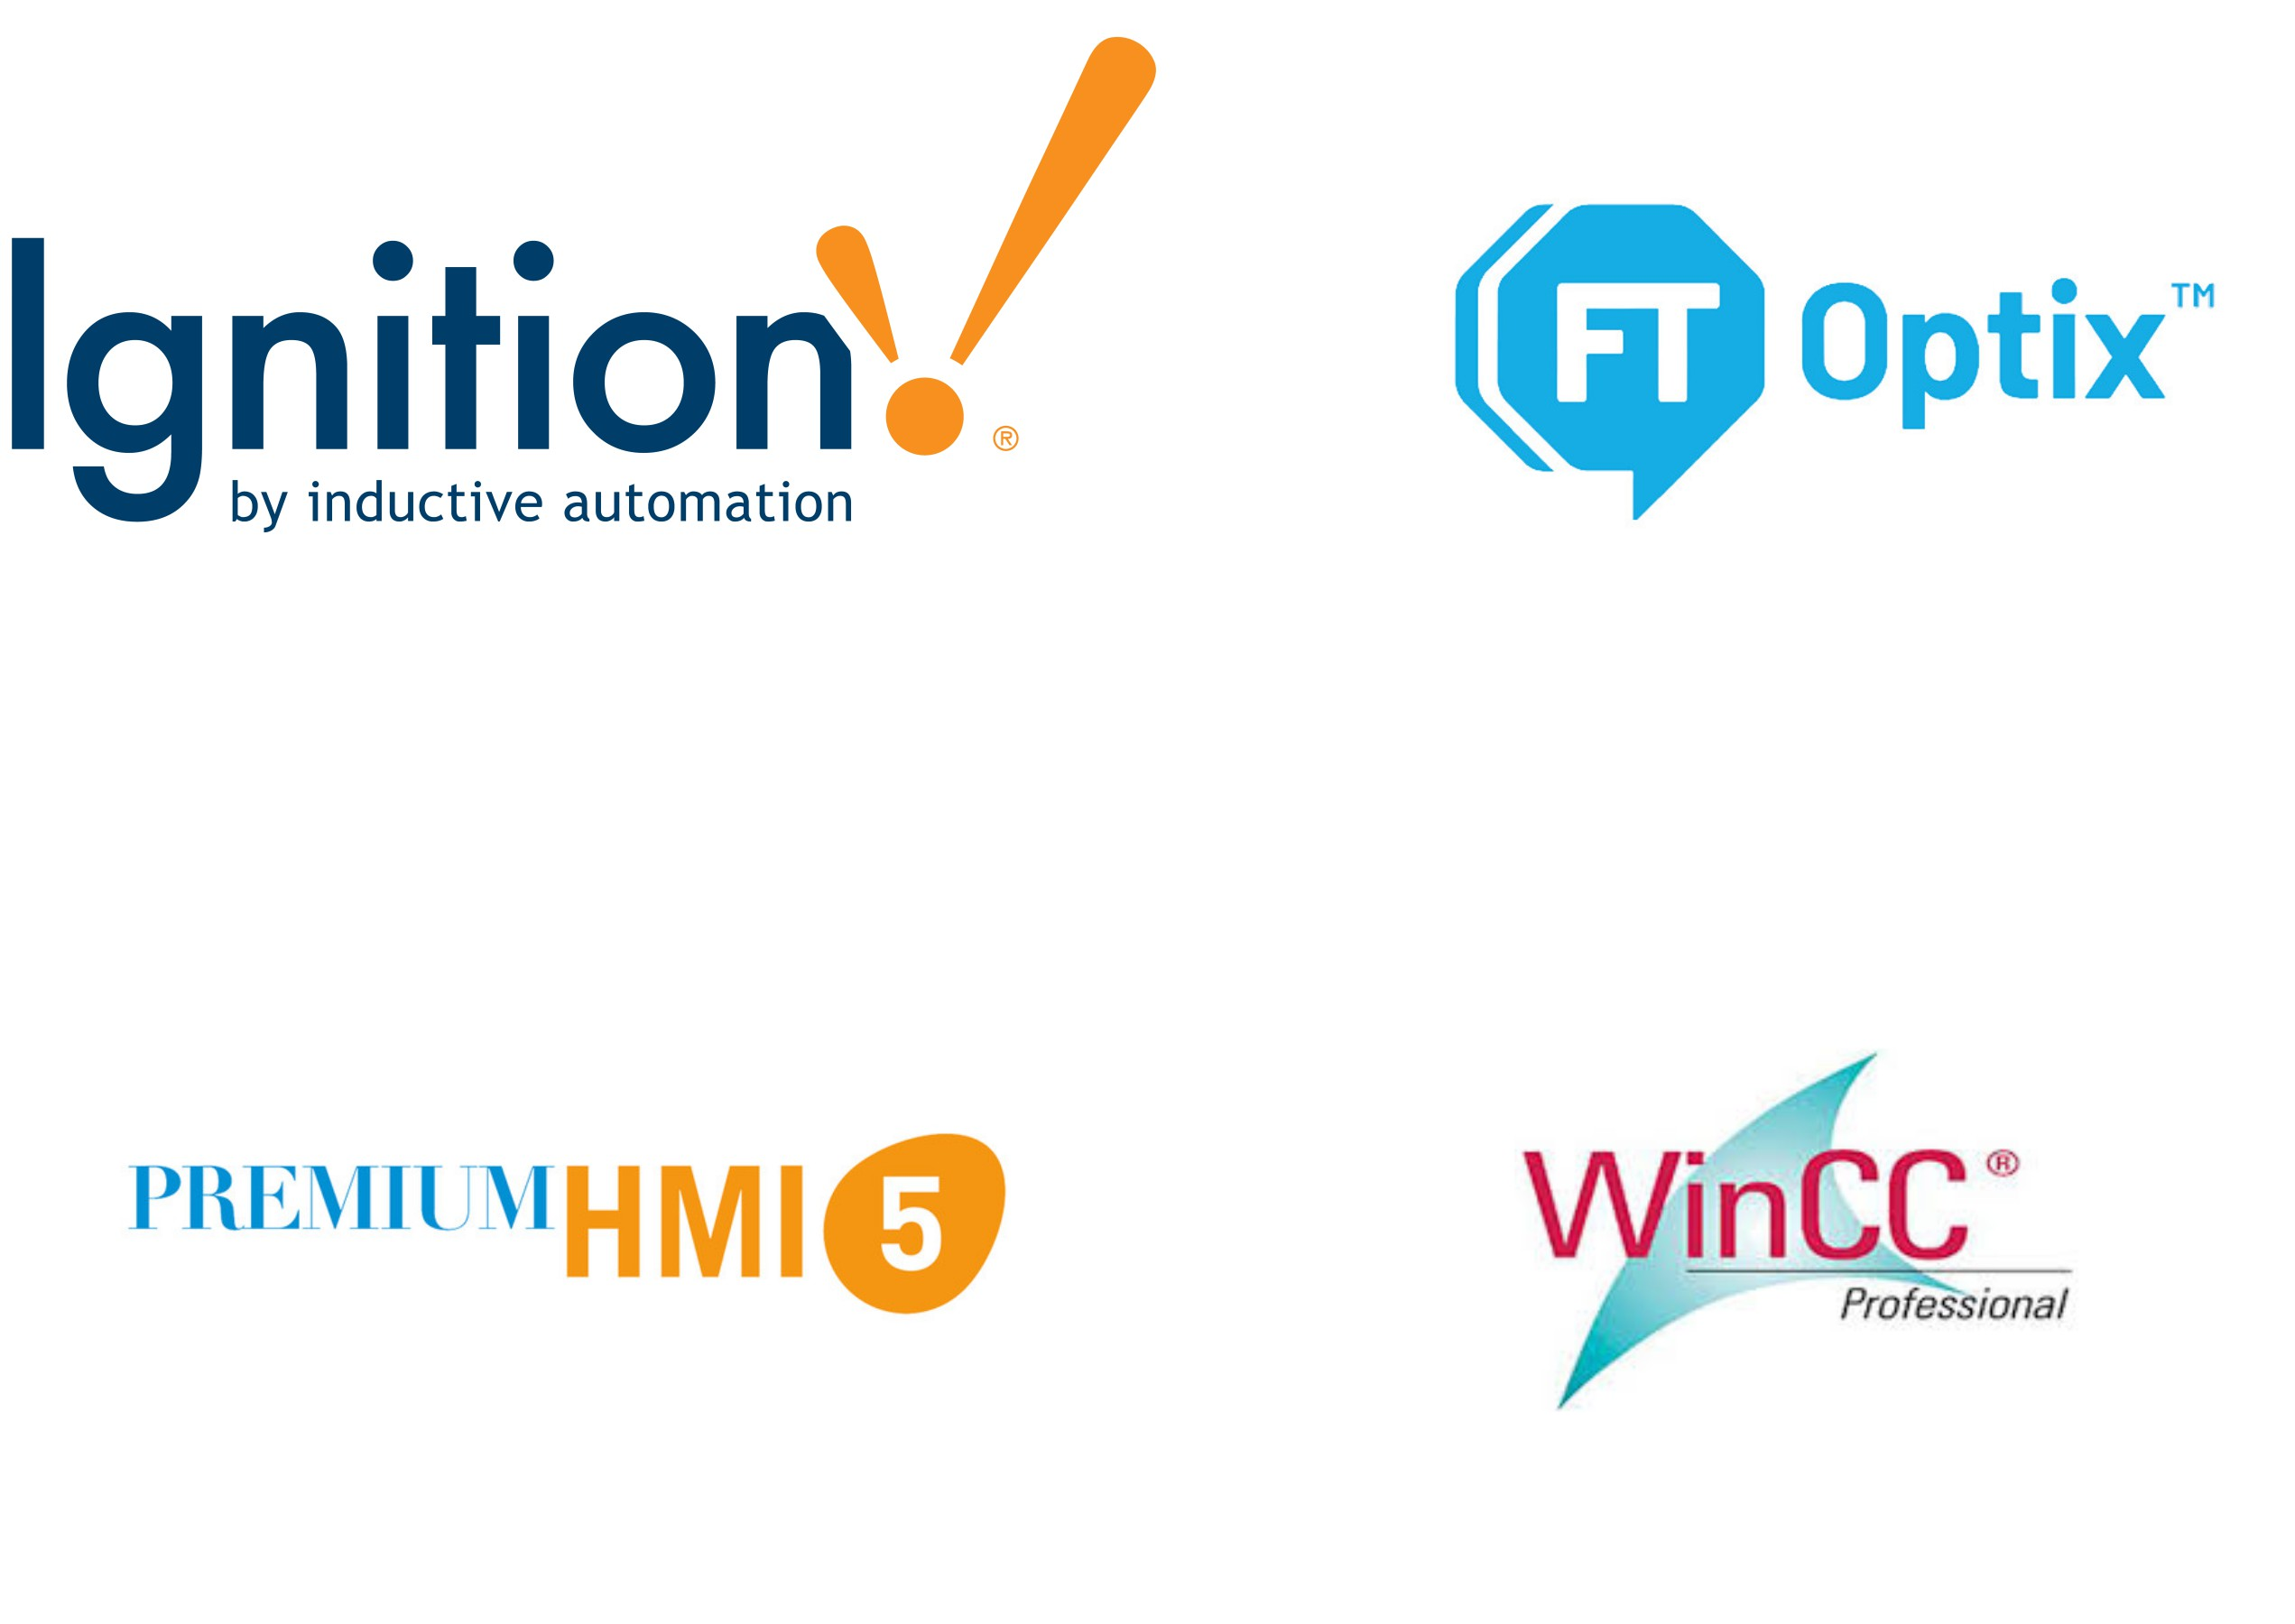
\includegraphics[width=0.5\linewidth]{Immagini/loghi.jpg}
    \caption{Esempi software per progettazione HMI}
    \label{fig:loghi.jpg}
\end{figure}

Ognuna di queste piattaforme possiede logiche diverse per poter progettare uno SCADA, nel mio caso è stata scelta come piattaforma FactoryTalk® Optix™, neo-piattaforma sviluppata da ASEM by Rockwell-Automation: 

\begin{displayquote}
    \textit{È l’innovativa piattaforma software perfetta per realizzare HMI moderne e responsive, con un’esperienza utente di alto livello, Gateway IIoT, applicazioni Edge Computing e in generale soluzioni legate alle esigenze dell’Industry 4.0.} \\ \textit{Grazie ad un’architettura completamente modulare ed estremamente flessibile sviluppata con tecnologie cross-platform, FT Optix™ permette di realizzare applicazioni compatibili con piattaforme ARM e x86 con sistemi operativi Windows e Linux, garantendo la massima flessibilità ai progettisti, che possono scegliere la piattaforma che meglio si adatta all’applicazione.} \\ \textit{FT Optix™ fa parte della suite cloud-based FactoryTalk® Design Hub™, che permette al team di progettazione di collaborare allo sviluppo dell’applicazione HMI tramite un sistema di controllo di versione distribuito, semplificando la gestione del software, aumentando la produttività ed accelerando il time to market.}\textsuperscript{\cite{asemautomation}}
\end{displayquote}

La scelta di approcciare a questa piattaforma di sviluppo è nata dal fatto che in REA l'innovazione è alla base della politica aziendale e il passaggio ad un nuovo software rappresenta la scelta perfetta per rimanere al passo con i tempi. Il software possiede un'interfaccia simile alle altre controparti ma con l'aggiunta che per SCADA più avanzati è possibile sfruttare l'uso di C\# in ambienti di sviluppo basati su .NET. Oltre a questo ho dovuto interfacciarmi con diversi software e librerie per poter far funzionare lo SCADA. 
Sul fronte C\# e ambiente di sviluppo, la scelta è ricaduta su Visual Studio Community per l'ampia customizzazione e il supporto continuo da parte di Microsoft. Inoltre per quanto riguarda la gestione di tutti i dati interni allo SCADA, due sono state le scelte su cui lavorare:
\begin{enumerate}
    \item Database locale di Optix™: per creare e gestire il database in SQLite e con l'ausilio di DB4S, è stato possibile interfacciarsi anche con le macchine più datate.
    \item Microsoft SQL Server Management Studio (SSMS): applicativo utilizzato già in REA per gestire vari database lato Server per gli impianti più complessi.
\end{enumerate}
Infine per il controllo delle versioni del progetto, data l'integrazione tra FT Optix™ e Git, la scelta è ricaduta su Git per tenere traccia di tutte le varie versioni dello SCADA durante lo sviluppo, eventualmente collaborare con altri sviluppatori e mantenere uno storico delle revisioni. 

\subsection{Lista Software utilizzati}
Ecco la lista dei software utilizzati durante la progettazione del sistema SCADA durante il tirocinio:
\begin{itemize}
    \item \textbf{FT Optix™}: versione 1.4.2.3
    \item \textbf{Microsoft Visual Studio 2022}: versione 17.11
    \item \textbf{Microsoft SQL Server Management Studio (SSMS)}: versione 20
    \item \textbf{DB Browser for SQLite (DB4S)}: versione 3.13.0
    \item \textbf{Git}: versione 2.47.0, direttamente da \textbf{GitHub Desktop}
\end{itemize}

\subsection{Struttura Generale di FactoryTalk Optix™}
FT Optix™ è un software strutturato per fornire modularità ai componenti utilizzati affinché i progetti possano essere suddivisi in componenti riutilizzabili, ciascuno con logica indipendente, e che possono essere richiamati in più parti dell'applicazione. Inoltre, come già anticipato, permette la gestione dei progetti multi-utente: con supporto per lo sviluppo collaborativo grazie al versionamento e controllo delle modifiche, oltre al supporto per protocolli industriali, come OPC UA, Modbus TCP/RTU, Ethernet/IP e altri standard di automazione. Altra caratteristica del software è la struttura a incapsulamento dei sinottici: come nella programmazione ad oggetti, viene sfruttato un tipo di design gerarchico, dove sono presenti oggetti grafici compositi, definiti Sinottici. Questi includono componenti nidificate con proprietà specifiche, logiche ed eventi. Inoltre, è possibile creare dei template parametrizzati per simulare macchinari, sensori o attuatori. Tutti questi oggetti grafici possono essere salvati in librerie condivise e riutilizzati in progetti diversi, riducendo tempi di sviluppo e migliorando la consistenza, oltre al fatto che è possibile utilizzare controlli avanzati come grafici, griglie e dashboard dinamiche per avere maggior controllo durante la progettazione. Infine, è possibile sfruttare sinottici reattivi - permettendo l'adattamento a diverse risoluzioni e formati dei pannelli HMI - e associare eventi o trigger ad ogni oggetto per eseguire azioni come aggiornamenti in tempo reale, invio di allarmi o gestione degli errori. Dal lato usabilità, fornisce simulazione attraverso ambiente di sviluppo, ossia è in grado di simulare il progetto completo con dati fittizi prima della messa in servizio, oltre a strumenti integrati per il debugging e la risoluzione di problemi, con visualizzazione di log e delle variabili in tempo reale.

\begin{figure} [ht]
    \centering
    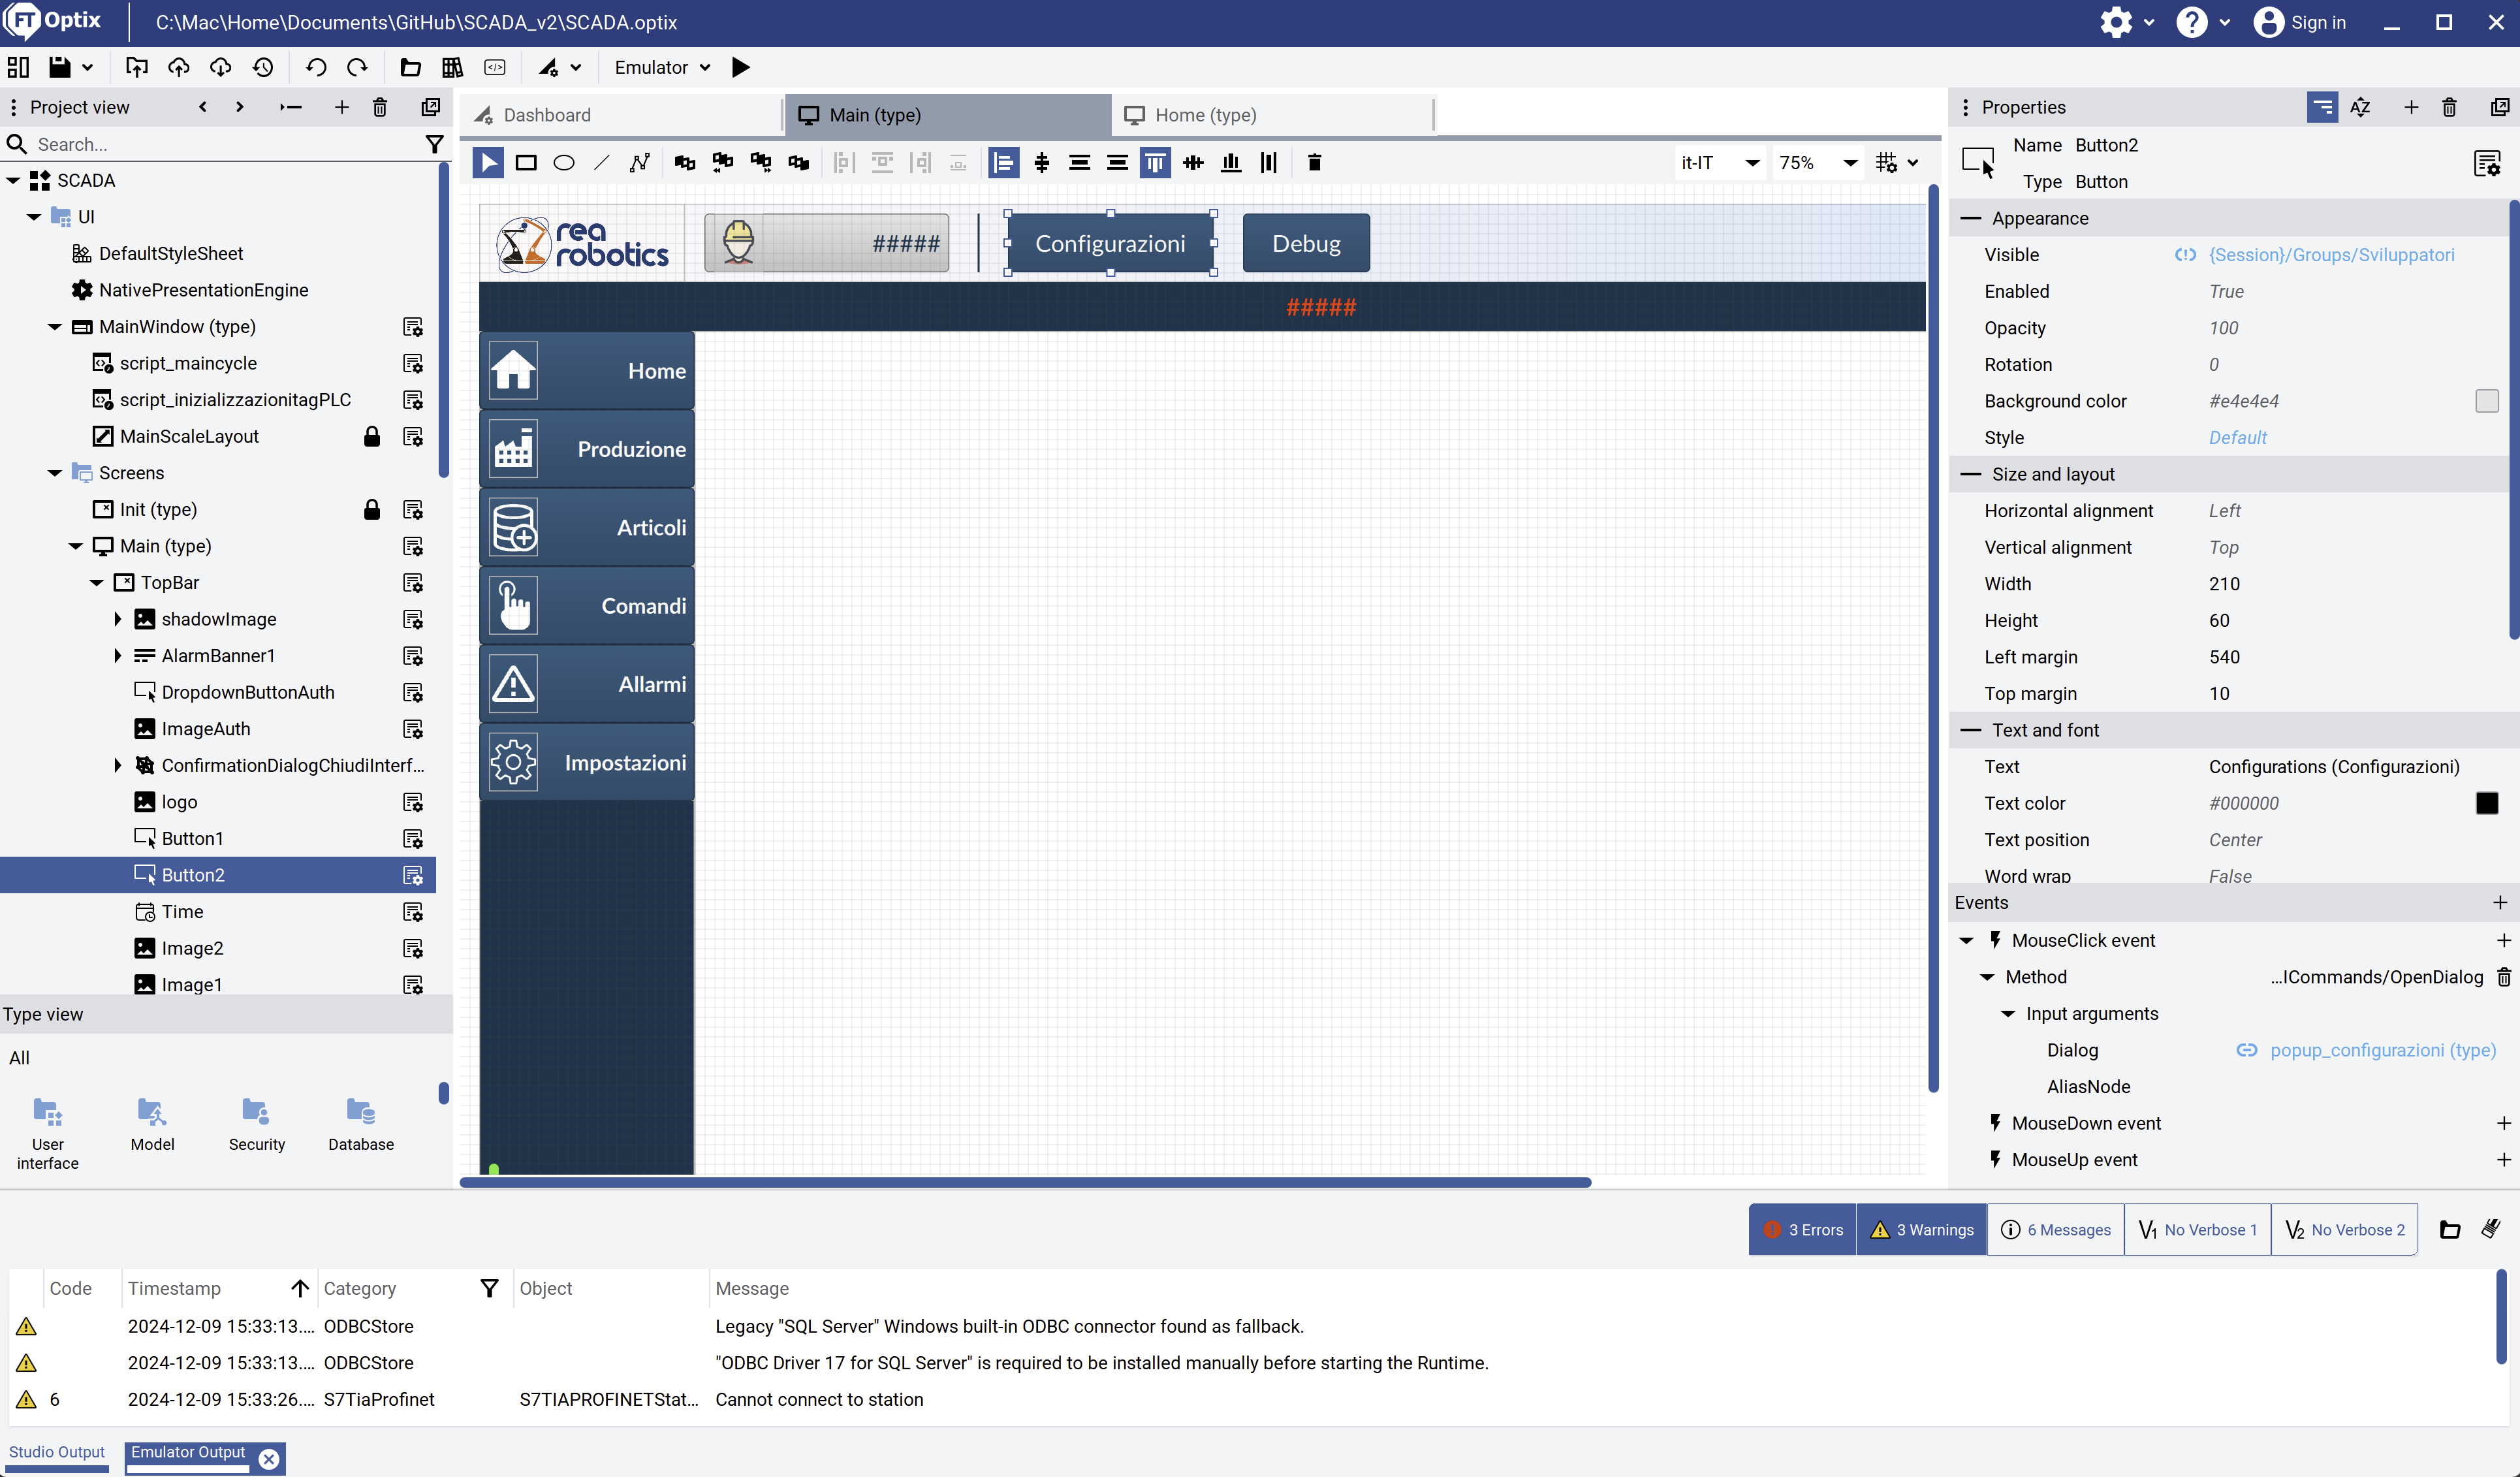
\includegraphics[width=0.5\linewidth]{Immagini/dashboard.png}
    \caption{Illustrazione dashboard di progetto}
    \label{fig:dashboard.png}
\end{figure}